\documentclass{uulm-assignment}

\faculty{}
\course{Höhere Mathematik 1}
\semester{\hspace{0.05cm}WiSe 2024/25}
\supervisor{\hspace{4.55cm} Benjamin Chladni - 1115697} %\students hat die formatierung rausgehauen :(


\assignmentno{}
\title{Blatt No. 3}


%%%%%%%%%%%%%%%%%%%%%%%%%%%%%%%%%%%%%%%%%%%%%%%%%%%%%%%%%%%%%%%%%%%%%%
% THE DOCUMENT BEGINS             	                              	 %
%%%%%%%%%%%%%%%%%%%%%%%%%%%%%%%%%%%%%%%%%%%%%%%%%%%%%%%%%%%%%%%%%%%%%%
\begin{document}
    \pagenumbering{roman}
    \maketitle
    
    \tableofcontents
	
    \newpage
    \pagenumbering{arabic}

    \section{Aufgabe 1}
    \subsection{a)}
        \subsubsection{}
            $$\text{Nullstellen von }f(x) = x^6 - x^2 \text{ in Wolframalpha: }$$
            \begin{center}
                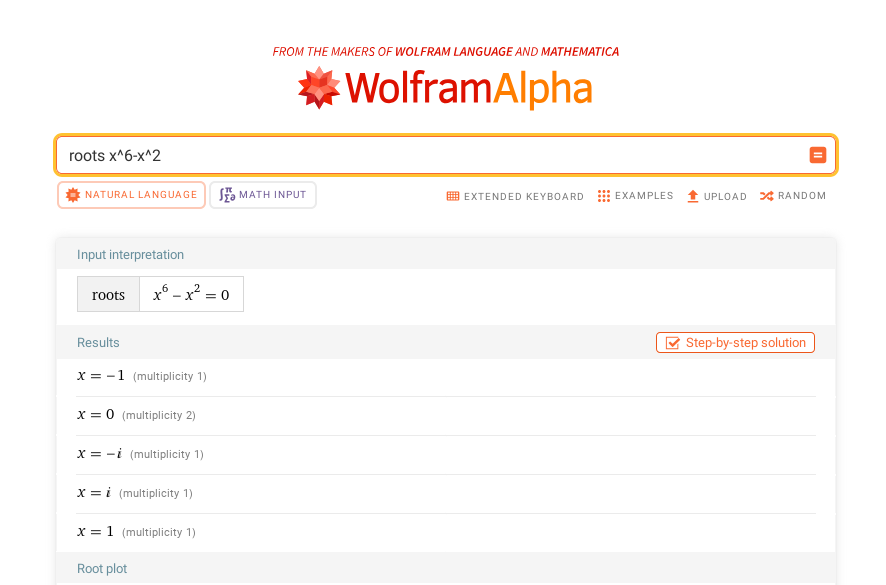
\includegraphics[width = 0.75\textwidth]{Aufgaben/01/1a)i).png}    
            \end{center}

        \subsubsection{}
            $$\text{Nullstellen von }f(x) = x^3 + 4x^2 - 7x + 2 \text{ in Wolframalpha: }$$
            \begin{center}
                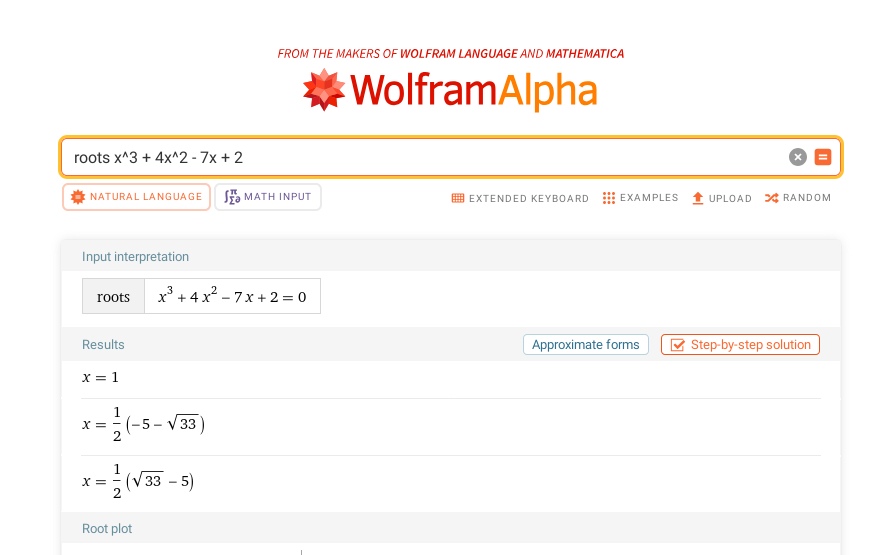
\includegraphics[width = 0.75\textwidth]{Aufgaben/01/1a)ii).png}    
            \end{center}
    \subsection{b)}
        $$\text{Potenzreihe von }a^x \text{ für } a>0, a\in \mathbb{R} \text{ in Wolframalpha: }$$
            \begin{center}
                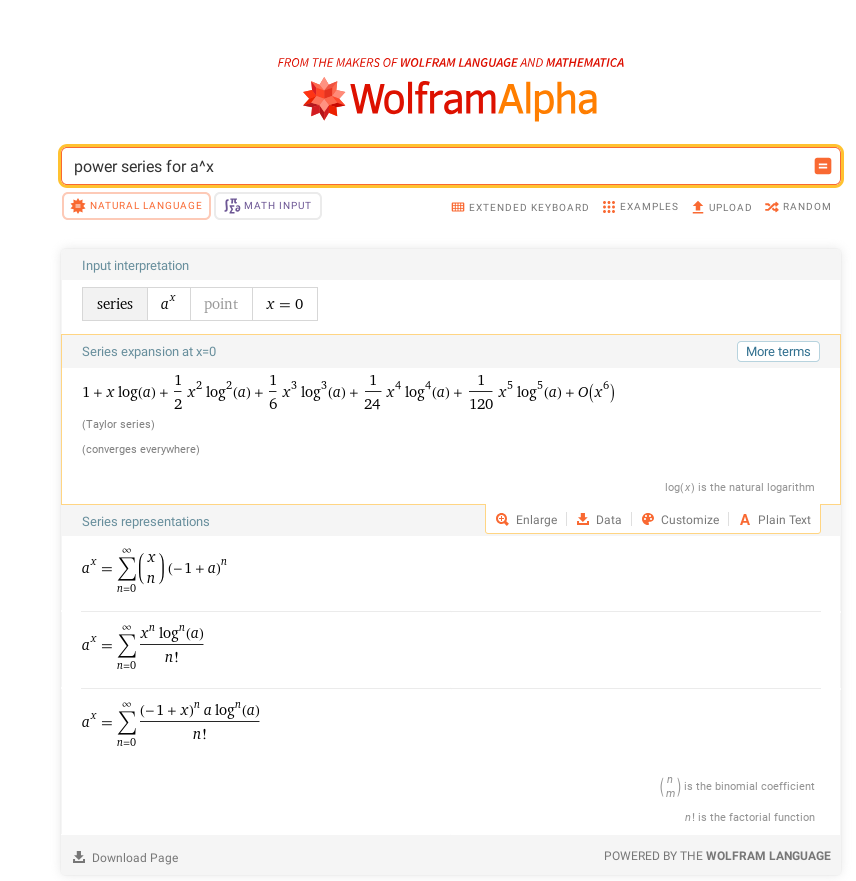
\includegraphics[width = 0.75\textwidth]{Aufgaben/01/1b).png}    
            \end{center}

        Da diese Potenzreihe für alle $a \in \mathbb{R}$ gilt, gilt diese analog auch für $a>0$

            
    \newpage

    \section{Aufgabe 2}
Sei $a \neq 0$
$$\Rightarrow ax^2+bx+c = 0$$
$$\Leftrightarrow ax^2+bx = -c$$
$$\Leftrightarrow x^2 + \frac{b}{a}x = - \frac{c}{a}$$
$$\Leftrightarrow x^2 + \frac{b}{a}x + (\frac{b}{2a})^2 = -\frac{c}{a} + (\frac{b}{2a})^2 $$
$$\Leftrightarrow (x+\frac{b}{2a})^2 = \frac{b^2}{4a^2} - \frac{c\cdot 4a}{a\cdot 4a}$$
$$\Leftrightarrow (x+\frac{b}{2a})^2 = \frac{b^2}{4a^2} - \frac{c\cdot 4a}{4a^2}$$
$$\Leftrightarrow (x+\frac{b}{2a})^2 = \frac{b^2-4ac}{4a^2}$$
$$\Leftrightarrow x+\frac{b}{2a} = \pm \sqrt{\frac{b^2-4ac}{4a^2}}$$
$$\Leftrightarrow x = \frac{-b}{2a} \pm \sqrt{\frac{b^2-4ac}{4a^2}}$$
$$\Leftrightarrow x_{1, 2} = \frac{-b}{2a} \pm \frac{\sqrt{b^2-4ac}}{2a}$$
$$\Leftrightarrow x_{1, 2} = \frac{-b \pm \sqrt{b^2-4ac}}{2a}$$
Da falls $a = 0$ das Polynom nicht mehr ein Polynom des zweiten Grades ist, fällt dieser Fall im Normalfall weg. Allerdings wurde ich darauf hingewiesen dass wir dies trotzdem herleiten sollen. \\
Sei $a = 0$
$$\Rightarrow ax^2+bx+c = 0$$
$$\Leftrightarrow bx+c = 0$$
$$\Leftrightarrow bx = -c$$
$$\Leftrightarrow x = -\frac{b}{c}$$
    \newpage

    \section{Aufgabe 3}
    \subsection{a)}
        $$f(x) = 0 \Leftrightarrow x^6-x^2 = 0$$
        $$\Leftrightarrow x^2(x^4-1) = 0$$
        $$\Leftrightarrow x^2(x^2-1)(x^2+1) = 0$$
        $$\Leftrightarrow x^2(x^2+1)(x+1)(x-1) = 0$$
        $\Rightarrow x_1 = 0, x_2 = -1, x_3 = 1, x_4 = i, x_5 = -i$

    \subsection{b)}
        $$f(x) = 0 \Leftrightarrow x^3+4x^2-7x+2 = 0$$
        Durch geschicktes Hinsehen bekommen wir $x_1 = 1$, wodurch wir im folgenden Schritt den Term aufteilen können in:
        $$\Rightarrow (x-1)(x^2+5x-2) = 0$$
        $$\Rightarrow (x-1) = 0 \lor x^2+5x-2 = 0$$
        $$\Rightarrow x_{2,3} = \frac{-5 \pm \sqrt{5^2-4\cdot 1 \cdot (-2)}}{2}$$
        $$\Leftrightarrow x_{2,3} = \frac{-5 \pm \sqrt{33}}{2}$$
        $$\Rightarrow x_2 = \frac{-5 + \sqrt{33}}{2} \land x_3 = \frac{-5 - \sqrt{33}}{2}$$
        
    \newpage

    \section{Aufgabe 4}
Wir wissen bereits: $cosh(x) = \frac{e^x+e^{-x}}{2}$ und wir wissen auch $ e^x = \sum_{n=0}^{\infty}\frac{x^n}{n!}$. \\
Wir wollen nun diese beiden Gleichungs so kombinieren, dass wir $cosh(x) = \sum_{i=0}^{\infty} \frac{x^{2n}}{2n!} $ bekommen
$$\Rightarrow 
cosh(x) = \frac{e^x+e^{-x}}{2} 
= \frac{\sum_{n=0}^{\infty}\frac{x^n}{n!} + \sum_{n=0}^{\infty}\frac{-x^n}{n!}}{2} 
$$
$$
= \frac{\sum_{n=0}^{\infty}\frac{x^2n}{2n!} + \sum_{n=0}^{\infty}\frac{x^2n+1}{(2n+1)!} + \sum_{n=0}^{\infty}\frac{x^2n}{2n!} - \sum_{n=0}^{\infty}\frac{x^2n+1}{(2n+1)!}}{2}
$$
$$= \frac{2 \cdot \sum_{n=0}^{\infty}\frac{x^2n}{2n!} }{2} = \sum_{n=0}^{\infty}\frac{x^2n}{2n!}$$
$$\Rightarrow cosh(x) = \sum_{n=0}^{\infty}\frac{x^2n}{2n!}$$
    \newpage

    \section{Aufgabe 5}
Wir können $a^x$ umschreiben zu $e^{x \cdot ln(a)}$ und wir wissen $e^x = \sum_{n=0}^{\infty} \frac{x^n}{n!}$ \\
$$\Rightarrow a^x = \sum_{n=0}^{\infty} \frac{(ln(a) \cdot x)^n}{n!}$$
    \newpage

    \section{Aufgabe 6}
Wir wollen \(((x^2 + y^2)^2 - 2a^2(x^2 - y^2) = 0)\) in Polarkoordinaten umformen. Dafür nutzen wir:
$$x = r \cos(\theta) \quad \text{und} \quad y = r \sin(\theta)$$
$$\Rightarrow ((r^2)^2 - 2a^2(r^2 \cos(2\theta)) = 0$$
$$\Leftrightarrow r^4 - 2a^2 r^2 \cos(2\theta) = 0$$
$$\Leftrightarrow r^2(r^2 - 2a^2 \cos(2\theta)) = 0$$
Dadurch bekommen wir: \(r = 0 \land r^2 = 2a^2 \cos(2\theta) \)
$$ \Rightarrow r = \sqrt{2}a \sqrt{\cos(2\theta)}$$

    \newpage

    \section{Aufgabe 7}
Wir wollen die Kurve $ x(t) = a(1 + t), y(t) = at^3$ der Parameterdarstullung in die Form $y = f(x)$ bringen
$$ \Rightarrow x = a(1 + t) \Rightarrow t = \frac{x}{a} - 1$$
$$\Rightarrow y = a\left(\frac{x}{a} - 1\right)^3 $$
$$ \Leftrightarrow y = a\left(\frac{x - a}{a}\right)^3 = \frac{(x - a)^3}{a^2}$$

Somit ist die Kurve in der Darstellung \( y = f(x) \):
$$
y = \frac{(x - a)^3}{a^2}
$$

    \newpage

    \section{Aufgabe 8}
Wir wählen $t = log(x)$
$$\Rightarrow x = e^t$$
$$\Rightarrow y = log(x)(log(x)+1) \Leftrightarrow y = t(t+1) = t^2 + t $$
Somit bekommen wir die Parameterdarstellung der Kurve:
$$x(t) = e^t$$
$$y(t) = t^2 + t$$
Dies gilt für $t \in \mathbb{R}$
    \newpage

    \section{Aufgabe 9}
    \subsection{a)}
        Gegeben ist die Kurve in Polarkoordinaten:
        $$r = \frac{4}{\sqrt{12 - 8 \sin^2(\varphi)}}$$
        Wir möchten diese Kurve in kartesische Koordinaten $(x, y)$ umschreiben. Dazu verwenden wir die bekannten Beziehungen zwischen Polarkoordinaten und kartesischen Koordinaten:
        \begin{align*}
            x &= r \cos(\varphi), \\
            y &= r \sin(\varphi), \\
            r^2 &= x^2 + y^2.
        \end{align*}
        
        Da $\sin(\varphi) = \frac{y}{r} $:
        $$\Rightarrow r = \frac{4}{\sqrt{12 - 8 \left(\frac{y}{r}\right)^2}}.$$
        $$\Leftrightarrow r^2 = \frac{16}{12 - 8 \frac{y^2}{r^2}}.$$
        $$\Leftrightarrow r^2 \left(12 - 8 \frac{y^2}{r^2}\right) = 16.$$
        $$\Leftrightarrow 12 r^2 - 8 y^2 = 16.$$
        $$\text{Da } r^2 = x^2 + y^2 \Rightarrow 12(x^2 + y^2) - 8 y^2 = 16.$$
        $$\Rightarrow 12x^2 + 4y^2 = 16.$$
        $$ \Rightarrow \frac{3x^2}{4} + \frac{y^2}{4} = 1.$$
        Dies ist die Gleichung einer Ellipse in kartesischen Koordinaten:
        $$\Rightarrow \frac{x^2}{\frac{4}{3}} + \frac{y^2}{4} = 1.$$

        Die Kurve in kartesischen Koordinaten ist also eine Ellipse mit Halbachsen \(\sqrt{\frac{4}{3}}\) entlang der \(x\)-Achse und \(2\) entlang der \(y\)-Achse.
    \subsection{b)}
        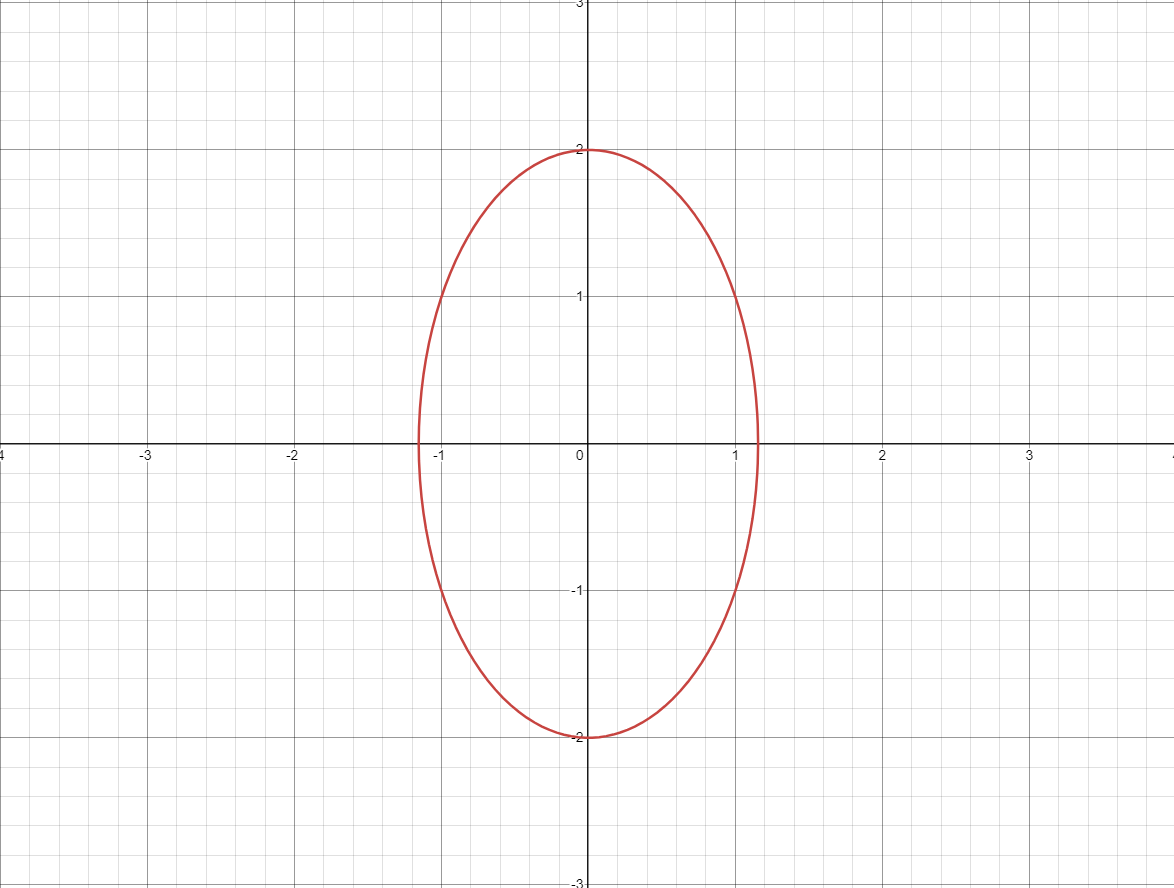
\includegraphics[width=\textwidth]{Aufgaben/09/9b).png}
    \newpage

    \section{Aufgabe 10}
$$z = \frac{(5+2i)(4-i)}{1+2i}$$
$$= \frac{(5+2i)(4-i)(1-2i)}{(1+2i)(1-2i)}$$
$$= \frac{(20-5i+8i-2i^2)(1-2i)}{1+2i-2i-4i^2}$$
$$= \frac{20-40i-5i+10i^2+8i-16i^2-2i^2-4i^3}{1+4}$$
$$= \frac{20-40i-5i-10+8i+16+2-4i}{5}$$
$$= \frac{28-41i}{5}$$
$$= \frac{28}{5}-\frac{41}{5}i$$
    \newpage

    \section{Aufgabe 11}
Wir müssen zuerst $2-i2\sqrt{3}$ in die Form $re^{i\phi}$ Umrechnen
$$r = \sqrt{2^2 - i^2 (2\sqrt{3})^2} = \sqrt{4+(2\sqrt{3})^2}=\sqrt{4+4\cdot3}=\sqrt{4+12}=\sqrt{16}=4$$
$$\phi = arctan(\frac{-2\sqrt{3}}{2}) = arctan(-\sqrt{3}) = -\frac{\pi}{3}$$
$$\Rightarrow 2-i2\sqrt{3} = 4exp(\frac{-i\pi}{3})$$
Wir berechnen nun den Betrag und das Argument der füfnten Wurzeln: 
$$r^{\frac{1}{4}}=4^{\frac{1}{5}}$$
und
$$arg=\frac{-\pi}{3 \cdot 5}+\frac{2\pi k}{5} \text{ für } k=0,1,2,3,4$$
$\Rightarrow$ Jede fünfte Wurzel hat die Form $z_k = 4^{\frac{1}{5}}e^{i(\frac{-\pi}{15}+\frac{2\pi k}{5})}$ für $k=0,1,2,3,4$. Also Rotieren wir den Winkel um $\frac{2\pi}{5}$ für jede Nachfolgende Wurzel
$$k=0 \Rightarrow \text{fünfte Wurzel: } 4^{\frac{1}{5}}e^{i(\frac{-\pi}{15})}$$
$$k=1 \Rightarrow \text{fünfte Wurzel: } 4^{\frac{1}{5}}e^{i(\frac{-\pi}{15}+\frac{2\pi}{5})}$$
$$k=2 \Rightarrow \text{fünfte Wurzel: } 4^{\frac{1}{5}}e^{i(\frac{-\pi}{15}+\frac{4\pi}{5})}$$
$$k=3 \Rightarrow \text{fünfte Wurzel: } 4^{\frac{1}{5}}e^{i(\frac{-\pi}{15}+\frac{6\pi}{5})}$$
$$k=4 \Rightarrow \text{fünfte Wurzel: } 4^{\frac{1}{5}}e^{i(\frac{-\pi}{15}+\frac{8\pi}{5})}$$
    \newpage

    \section{Aufgabe 12}
Der Rot markierte Teil der Menge ist in M: \\
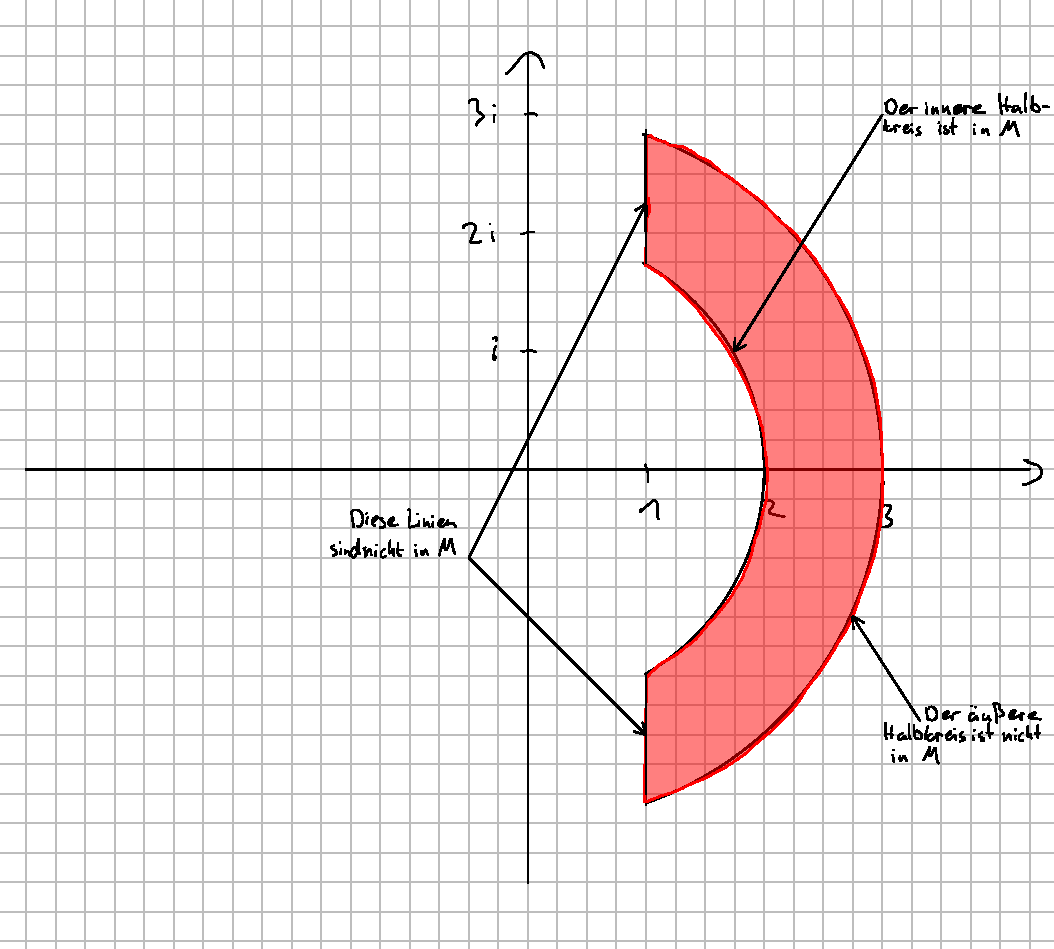
\includegraphics[width=\textwidth]{Aufgaben/12/Skizze_HM_12.pdf}

        
\end{document}